 \iffalse
\let\negmedspace\undefined
\let\negthickspace\undefined
\documentclass[journal,12pt,twocolumn]{IEEEtran}
\usepackage{cite}
\usepackage{amsmath,amssymb,amsfonts,amsthm}
\usepackage{algorithmic}
\usepackage{graphicx}
\usepackage{textcomp}
\usepackage{xcolor}
\usepackage{txfonts}
\usepackage{listings}
\usepackage{enumitem}
\usepackage{mathtools}
\usepackage{gensymb}
\usepackage{comment}
\usepackage{tikz}
\usepackage[breaklinks=true]{hyperref}
\usepackage{tkz-euclide} 
\usepackage{listings}
\usepackage{gvv}
\def\inputGnumericTable{}
\usepackage[latin1]{inputenc}                              
\usepackage{color}                                            
\usepackage{array}                                            
\usepackage{longtable}                                       
\usepackage{calc}                                             
\usepackage{multirow}                                         
\usepackage{hhline}                                           
\usepackage{ifthen}                                           
\usepackage{lscape}

\newtheorem{theorem}{Theorem}[section]
\newtheorem{problem}{Problem}
\newtheorem{proposition}{Proposition}[section]
\newtheorem{lemma}{Lemma}[section]
\newtheorem{corollary}[theorem]{Corollary}
\newtheorem{example}{Example}[section]
\newtheorem{definition}[problem]{Definition}
\newcommand{\BEQA}{\begin{eqnarray}}
\newcommand{\EEQA}{\end{eqnarray}}
\newcommand{\define}{\stackrel{\triangle}{=}}
\theoremstyle{remark}
\newtheorem{rem}{Remark}
\begin{document}

\bibliographystyle{IEEEtran}
\vspace{3cm}

\title{Discrete 10.5.3 Q-3}
\author{EE23BTECH11207 -KAILASH.C$^{*}$% <-this % stops a space
}
\maketitle
\newpage
\bigskip

\renewcommand{\thefigure}{\theenumi}
\renewcommand{\thetable}{\theenumi}

In an AP:
\begin{enumerate}
\item given a = 5, d = 3,$a_n=5$, find n and $S_n$.
\item given a = 7, $a_{13}$=35, find d and $S_{13}$.
\item given $a_{12}=37$, d = 3, find a and $S_{12}$.
\item given $a_3$= 15, $S_{10}$ = 125, find d and $a_{10}$.
\item given d = 5, $S_9$= 75, find a and $a_9$.
\item given a = 2, d = 8, $S_n$= 90, find n and $a_n$.
\item given a = 8, $a_n$= 62, $S_n$= 210, find n and d.
\item given an= 4, d = 2, $S_n=-14$, find n and a.
\item given a = 3, n = 8, $S_n$ = 192, find d.
\item given l = 28, S = 144, and there are total 9 terms. Find a.
\end{enumerate}\\
\solution
\fi
In the 9th subpart:
\begin{table}[h]
\begin{tabular}{|l|l|}
\hline
\textbf{Symbols} & \textbf{Definition}\\ \hline
$x\brak{0}$ & First term\\ \hline
d & Difference\\ \hline
$x\brak{n}$ & General term \\ \hline
$y\brak{n}$ & Sum of terms till $n_{th}$term \\ \hline
$X\brak{z}$ & Z-Transformation Of $x\brak{n}$\\ \hline
\end{tabular}
\caption{Definition Table}
\label{tab:ncert 10_5_3_3}
\end{table}

By using sum of n terms of A.P:
\begin{align}
y\brak{n}&=\frac{\brak{n+1}}{2}\brak{2x\brak{0}+nd}\label{eq:105331}\\
 192&=\frac{8}{2}\brak{2\brak{3}+7d}\label{eq:105332}\\
 48&=6+7d\label{eq:105533}\\
 d&=\frac{42}{7}\label{eq:105334}\\
 d&=6\label{eq:105335}
\end{align}
The general term is:
\begin{align}
    x\brak{n}&=\brak{3+6n}u\brak{n}\label{eq:105336}
\end{align}
From \eqref{eq:apz} For an AP,we get:
\begin{align}
    X\brak{z}&=\frac{6z^{-1}}{\brak{1-z^{-1}}^2}+\frac{3}{\brak{1-z^{-1}}}\label{eq:105337}
\end{align}
\begin{figure}[h]
        \centering
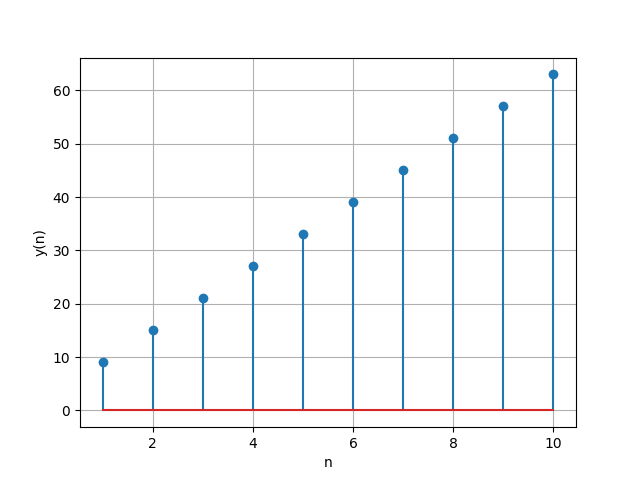
\includegraphics[width=\columnwidth]{ncert-maths/10/5/3/3/figs/Graphimage.png}
\caption{Graph of $x\brak{n}$ vs n}
\label{fig:Fig10_5_3_3}
\end{figure}

